\documentclass[12pt]{article}
\usepackage{sbc-template}
\usepackage{graphicx,url}
%\usepackage[brazil]{babel}   
\usepackage[utf8]{inputenc}  
\usepackage{listings}

\sloppy
\title{Simulador de Redes -- ARP e ICMP\\ Redes de Computadores I}
\author{João Pedro Chagas\inst{1}, Lásaro Curtinaz Dumer\inst{1}}
\address{Faculdade de Informática -- Pontifícia Universidade Católica do Rio Grande do Sul
 (UFRGS)\\
  Av. Ipiranga, 6681 Partenon -- 90.619-900 -- Porto Alegre -- RS -- Brasil
  \email{\{joao.chagas.001,lasaro.dumer\}@acad.pucrs.br}
}

\begin{document} 
\maketitle


%relatório (em pdf) contendo: 
%(i) detalhes de implementação (linguagem, classes, principais métodos); 
%(ii) descrição de como utilizar o simulador; 
%(iii) limitações do simulador implementado e dificuldades de implementação; 
%(iv) exemplo de execução com 1 topologia composta por no mínimo 3 roteadores

%\begin{abstract}
%\end{abstract}     
%\begin{resumo} 
%\end{resumo}
\section{Implementação}

Para que fosse possível realizar a atividade proposta, foi escolhida a linguagem de programação, para a implementação do simulador, C++, por ser uma linguagem multiplataforma, ser orientada a objetos e ter uma fácil manipulação de bits, algo que em pequenas tarefas nos foi muito útil. Para conseguir ao resultado da construção do simulador que estamos propondo, foi necessário, segundo nossa modelagem, a criação de 9 classes para que fosse possível realizar todas as operações descritas no enunciado da atividade.
[imagem diagrama de calsses]

\begin{figure}[ht]
\centering
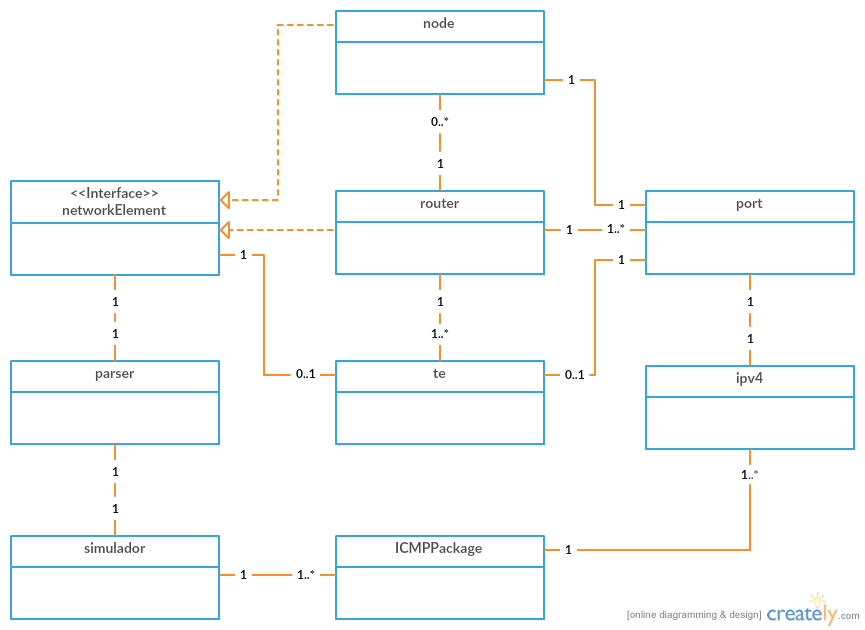
\includegraphics[width=1\textwidth]{DiagramaClasses.png}
\caption{Diagrama de classes}
\label{fig:DiagramaClasses}
\end{figure}

A classe simulador é a classe principal, ou seja, todas a execução acontece por ela, temos as classes dos objetos do modelo da rede, sendo assim \emph{router} sendo o roteador, \emph{port} sendo as portas do roteador, \emph{node} sendo os nodos da rede. \emph{Networkelements} e \emph{te} também são objetos do modelo de redes mas estes merecem uma explicação separada, \emph{networkelements} foi criado, pois ao longo do desenvolvimento do trabalho, notou-se que cada elemento (router e node) tinha seus métodos particulares mas invariavelmente todos tinha métodos de GET em comum, seja para pegar o nome ou o endereço IP. Sendo assim visando as boas práticas de programação criamos um objeto genérico no qual todos os demais o extenderiam, facilitando também na hora de trabalhar com\emph{buffer}, visto que todos a principio são objetos iguais. Já a \emph{te} é a classe que especifica as linhas da tabela de roteamento do roteador, ou seja, a tupla de rede  destino, \emph{nexthop} e porta é um objecto \emph{te}.


A classe \emph{ipv4} foi criada para representar um enddreço IP, por esta razão implementa alguns métodos para trabalhar com números binários baseados em endereços IPs, existem funções no arquivo \emph{util.hpp} contém alguns métodos que auxiliam no desenvolvimento de métodos mais importantes.


Porém as classes com métodos mais importantes são as classes \emph{parser} e \emph{ICMPPackage}, a primeira é responsável por, a partir do arquivo de entrada especificado, fazer a criação dos objetos do modelo da rede para que seja possível executar o comando descrito na chamada de execução do sistema. Já a classe ICMPPackage que representa os pacotes \emph{ICMP echo reply} e \emph{ICMP echo reply}, e executa fragmentação e remontagem, são basicamente os passos que fazem com que o sistema consiga executar o comando descrito na execução do programa. Porém estes métodos são chamados na classe \emph{simulador}, que como dito anteriormente é a principal e abriga o algoritmo de roteamento em si e que só consegue executá-lo utilizando o métodos descritos em outras classes mas principalmente os que foram desenvolvidos dentro do ICMPPackage.


\section{Utilização}
Para que seja possível executar o programa é necessário primeiramente compilar os arquivos dentro do pacote. Para facilitar esta tarefa existe, dentro do pacote, um \emph{makefile} com todas as compilações necessárias, sendo assim necessário apenas acessar a pasta raiz do pacote e executar o comando \emph{make}. Após isto todos os arquivos estarão prontos para utilização sendo necessário apenas executar o comando corretamente. Uma observação na descrição do comando, onde houver "[]" é onde deve ser substituído pela informação que se quer testar. Segue o comando de execução:


\begin{lstlisting}[breaklines=true,language=sh]
$ bin/simulador samples/[topologia.txt] [nodo_inicial] [nodo_final] [menssagem]
\end{lstlisting}


\section{Limitações e Dificuldades}
Durante o processo de desenvolvimento da ferramenta proposta foram encontradas algumas dificuldades que foram superadas, primeiramente começamos o desenvolvimento da aplicação na linguagem de programação Java, porém no decorrer foi notado que existiria a necessidade de operar bits e que isso em Java acrescentaria uma dificuldade que não havia necessidade de se enfrentar. Sendo assim para mitigar esse problema foi substituído o Java por C++. Em um segundo momento a dificuldade encontrada foi de como executar o processo de passar os pacotes entre os objetos da rede. As possibilidades encontradas foram através da recursão, descartada levando em consideração que o retorno do pacote poderia ser feito por um caminho diferente do que foi enviado o pacote. Sendo assim a solução encontrada foi utilizar um objeto genérico para executar as operações necessárias e verificar quando o mesmo chegou ao final e a utilização de um \emph{buffer} de \emph{requests} que necessitam serem processadas a cada novo estado.

\section{Execução}
Como exemplo de execução temos a rede abaixo e a saída do programa para o comando mencionado.

\begin{figure}[ht]
\centering
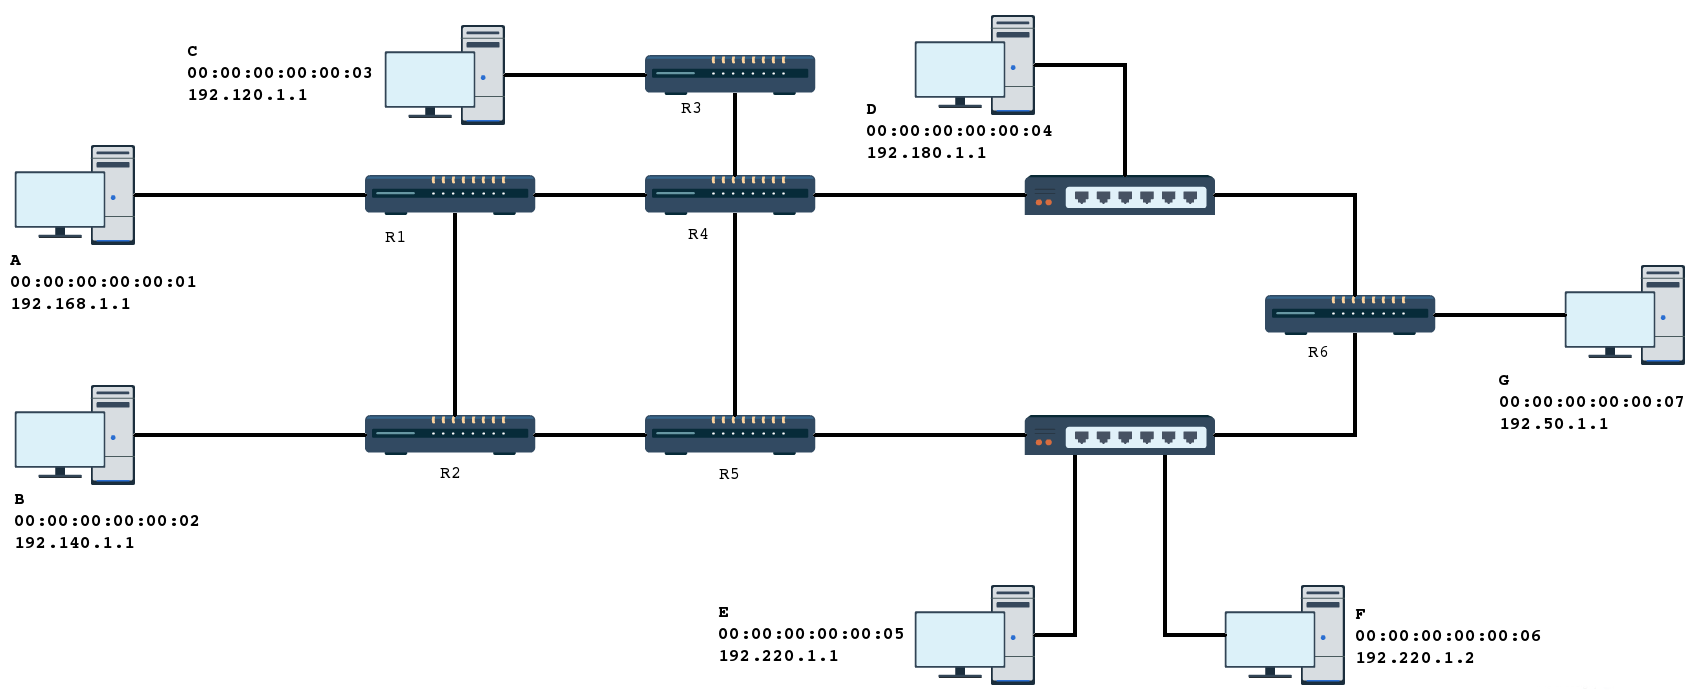
\includegraphics[width=1\textwidth]{NetworkDiagram_01.png}
\caption{Diagrama de rede}
\label{fig:NetworkDiagram_01}
\end{figure}
Comando:

\begin{lstlisting}[breaklines=true,language=sh]
$ bin/simulador samples/network_01.txt a g helloword
\end{lstlisting}


Saida:


\begin{lstlisting}[breaklines=true]
a box a : ARP - Who has 192.168.1.2? Tell 192.168.1.1;
r1 => a : ARP - 192.168.1.2 is at 00:00:00:00:01:01;
a => r1 : ICMP - Echo (ping) request (src=192.168.1.1 dst=192.50.1.1 ttl=8 data=helloword);
r1 box r1 : ARP - Who has 20.0.1.2? Tell 20.0.1.1;
r4 => r1 : ARP - 20.0.1.2 is at 00:00:00:00:03:04;
r1 => r4 : ICMP - Echo (ping) request (src=192.168.1.1 dst=192.50.1.1 ttl=7 data=helloword);
r4 box r4 : ARP - Who has 192.180.1.3? Tell 192.180.1.2;
r6 => r4 : ARP - 192.180.1.3 is at 00:00:00:00:05:05;
r4 => r6 : ICMP - Echo (ping) request (src=192.168.1.1 dst=192.50.1.1 ttl=6 data=helloword);
r6 box r6 : ARP - Who has 192.50.1.1? Tell 192.50.1.2;
g => r6 : ARP - 192.50.1.1 is at 00:00:00:00:00:07;
r6 => g : ICMP - Echo (ping) request (src=192.168.1.1 dst=192.50.1.1 ttl=5 data=hello);
r6 => g : ICMP - Echo (ping) request (src=192.168.1.1 dst=192.50.1.1 ttl=5 data=word);
g rbox g : Received helloword;
g => r6 : ICMP - Echo (ping) reply (src=192.50.1.1 dst=192.168.1.1 ttl=8 data=hello);
g => r6 : ICMP - Echo (ping) reply (src=192.50.1.1 dst=192.168.1.1 ttl=8 data=word);
r6 box r6 : ARP - Who has 192.220.1.3? Tell 192.220.1.4;
r5 => r6 : ARP - 192.220.1.3 is at 00:00:00:00:04:01;
r6 => r5 : ICMP - Echo (ping) reply (src=192.50.1.1 dst=192.168.1.1 ttl=7 data=hello);
r6 => r5 : ICMP - Echo (ping) reply (src=192.50.1.1 dst=192.168.1.1 ttl=7 data=word);
r5 box r5 : ARP - Who has 30.0.1.1? Tell 30.0.1.2;
r2 => r5 : ARP - 30.0.1.1 is at 00:00:00:00:02:03;
r5 => r2 : ICMP - Echo (ping) reply (src=192.50.1.1 dst=192.168.1.1 ttl=6 data=hello);
r5 => r2 : ICMP - Echo (ping) reply (src=192.50.1.1 dst=192.168.1.1 ttl=6 data=word);
r2 box r2 : ARP - Who has 10.0.1.1? Tell 10.0.1.2;
r1 => r2 : ARP - 10.0.1.1 is at 00:00:00:00:01:02;
r2 => r1 : ICMP - Echo (ping) reply (src=192.50.1.1 dst=192.168.1.1 ttl=5 data=hello);
r2 => r1 : ICMP - Echo (ping) reply (src=192.50.1.1 dst=192.168.1.1 ttl=5 data=word);
r1 => a : ICMP - Echo (ping) reply (src=192.50.1.1 dst=192.168.1.1 ttl=4 data=hello);
r1 => a : ICMP - Echo (ping) reply (src=192.50.1.1 dst=192.168.1.1 ttl=4 data=word);
a rbox a : Received helloword;
\end{lstlisting}

\subsection{Arquivo da topologia}
Abaixo segue o arquivo da topologia usada, para melhor visualização algumas tabulações foram adicionadas, mas o arquivo na integra será entregue junto a este relatório e estará com o nome \emph{network\_01.txt}.


\begin{lstlisting}[breaklines=true]
#NODE
A,00:00:00:00:00:01,192.168.1.1,20,192.168.1.2
B,00:00:00:00:00:02,192.140.1.1,20,192.140.1.2
C,00:00:00:00:00:03,192.120.1.1,5,192.120.1.2
D,00:00:00:00:00:04,192.180.1.1,50,192.180.1.2
E,00:00:00:00:00:05,192.220.1.1,30,192.220.1.3
F,00:00:00:00:00:06,192.220.1.2,30,192.220.1.3
G,00:00:00:00:00:07,192.50.1.1,5,192.50.1.2
#ROUTER
R1,3,
	00:00:00:00:01:01,192.168.1.2,20,
    00:00:00:00:01:02,10.0.1.1,10,
    00:00:00:00:01:03,20.0.1.1,10
R2,3,
	00:00:00:00:02:01,192.140.1.2,20,
    00:00:00:00:02:02,10.0.1.2,10,
    00:00:00:00:02:03,30.0.1.1,10
R3,2,
	00:00:00:00:02:01,192.120.1.2,5,
    00:00:00:00:02:02,40.0.1.1,40
R4,4,
	00:00:00:00:03:01,192.180.1.2,50,
    00:00:00:00:03:03,40.0.1.2,40,
    00:00:00:00:03:03,50.0.1.1,50,
    00:00:00:00:03:04,20.0.1.2,10
R5,3,
	00:00:00:00:04:01,192.220.1.3,30,
    00:00:00:00:04:04,30.0.1.2,10,
    00:00:00:00:04:03,50.0.1.2,50
R6,3,
	00:00:00:00:05:01,192.50.1.2,5,
    00:00:00:00:05:05,192.180.1.3,50,
    00:00:00:00:05:03,192.220.1.4,30
#ROUTERTABLE
R1,192.168.1.0,0.0.0.0,0
R1,10.0.1.0,0.0.0.0,1
R1,20.0.1.0,0.0.0.0,2
R1,192.140.1.0,10.0.1.2,1
R1,0.0.0.0,20.0.1.2,2
R2,192.140.1.0,0.0.0.0,0
R2,10.0.1.0,0.0.0.0,1
R2,30.0.1.0,0.0.0.0,2
R2,192.168.1.0,10.0.1.1,1
R2,0.0.0.0,10.0.1.1,1
R3,192.120.1.0,0.0.0.0,0
R3,40.0.1.0,0.0.0.0,1
R3,0.0.0.0,40.0.1.2,1
R4,192.180.1.0,0.0.0.0,0
R4,40.0.1.0,0.0.0.0,1
R4,50.0.1.0,0.0.0.0,2
R4,20.0.1.0,0.0.0.0,3
R4,192.168.1.0,20.0.1.1,3
R4,192.140.1.0,20.0.1.1,3
R4,192.120.1.0,40.0.1.1,1
R4,192.220.1.0,50.0.1.2,2
R4,192.50.1.0,192.180.1.3,0
R4,0.0.0.0,192.180.1.3,0
R5,192.220.1.0,0.0.0.0,0
R5,30.0.1.0,0.0.0.0,1
R5,50.0.1.0,0.0.0.0,2
R5,192.140.1.0,30.0.1.1,1
R5,192.180.1.0,50.0.1.1,2
R5,0.0.0.0,30.0.1.1,1
R6,192.50.1.0,0.0.0.0,0
R6,192.180.1.0,0.0.0.0,1
R6,192.220.1.0,0.0.0.0,2
R6,0.0.0.0,192.220.1.3,2
\end{lstlisting}

% \bibliographystyle{sbc}
% \bibliography{sbc-template}

\end{document}
